\documentclass[10pt,utf8]{beamer}

\mode<presentation> {
%  \usetheme{Boadilla}
  \usetheme{Madrid}
%	\usetheme{Fzu}
  \setbeamercovered{transparent}
}

\usepackage{palatino}
\usepackage{graphicx}
\usepackage{array}
\usepackage{color}
\usepackage{subfigure}
\usepackage{colortbl}
\usepackage{amsmath}
\usepackage{hyperref}
%\usepackage{tikz}
%\usetikzlibrary{arrows,shapes,backgrounds}


%\definecolor{MyDarkGreen}{rgb}{0.3,0.7,0.3}

\setbeamertemplate{caption}{\raggedright\insertcaption\par} %turn off caption prefix ("Figure")

\title{Infinispan}
\author{Vojtěch Juránek}
\institute[Red Hat]{JBoss - a division by Red Hat}
\date{11.~10.~2015, ACM RACS, Prague}

\newenvironment{mylisting}
{\begin{list}{}{\setlength{\leftmargin}{1em}}\item\scriptsize\bfseries}
{\end{list}}

\newenvironment{mytinylisting}
{\begin{list}{}{\setlength{\leftmargin}{1em}}\item\tiny\bfseries}
{\end{list}}


\begin{document}

%\tikzstyle{every picture}+=[remember picture]
%\tikzstyle{na} = [baseline=-.5ex]


\begin{frame}
 \titlepage
\end{frame}

\begin{frame}
	\frametitle{Data today}
	\begin{figure}
		\centering
		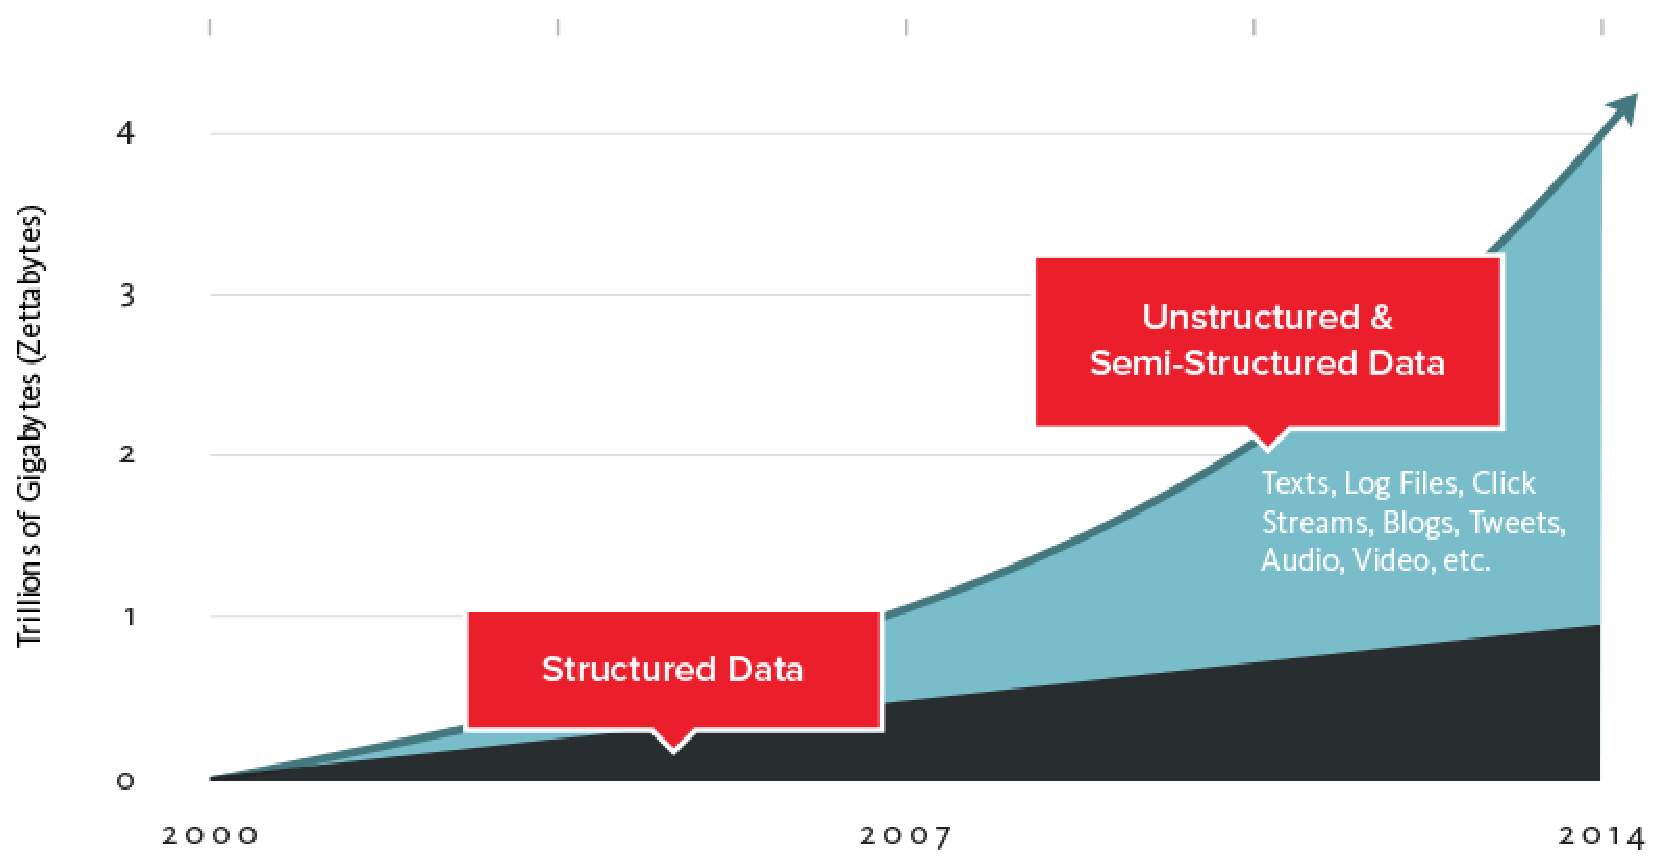
\includegraphics[width=10cm]{./img/why-nosql-2.eps}
		\caption{\tiny{Source: http://www.couchbase.com/nosql-resources/what-is-no-sql}}
	\end{figure}
\end{frame}

\begin{frame}
	\frametitle{Data today}
	\begin{itemize}
		\item Huge amount of data
		\begin{itemize}
			\item You can scale up, but sooner or later you'll need to scale out
			\item Need for highly scaleable solution also because of coste efectiveness
		\end{itemize}
		\item Lots of data is semi-structured or not structured at all (texts, log files, audio, video, click streams \dots)
		\begin{itemize}
			\item (spis kvuli performance) Needed ability to store unstructured data
			\item But ability  to talk to RDBMS is often needed as well
		\end{itemize}
	\end{itemize}
\end{frame}

\begin{frame}
	\frametitle{Why caching}
	\begin{figure}
		\centering
		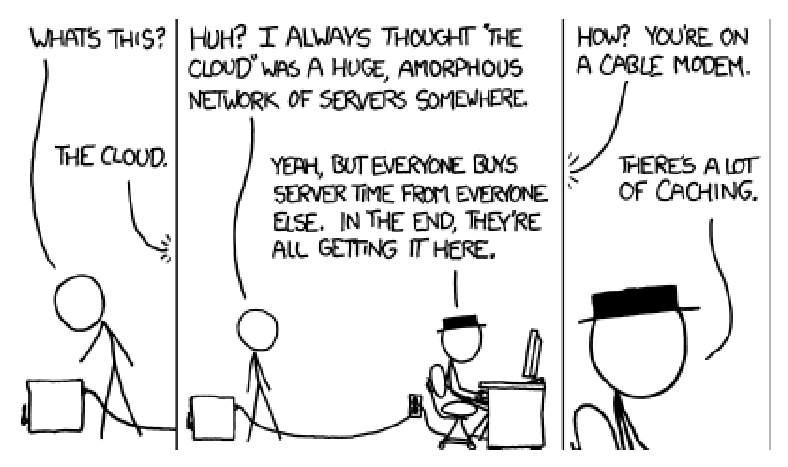
\includegraphics[width=12cm]{./img/xkcd_908.eps}
		\caption{\tiny{Source: Part of \href{http://xkcd.com/908/}{xkcd \#908}}}
	\end{figure}
\end{frame}

\begin{frame}
	\frametitle{Why in-memory}
	\begin{itemize}
	 \item Lots of data is needed in real-time (BigData $\rightarrow$ FastData)
	 \item Some tasks can be completed much faster when data are kept in memory
	 \item Keep data in memory during processing of whole application stack, not only during processing in one application in the stack
	 \item With data replication you can keep your data only in memory
	\end{itemize}
\end{frame}


\begin{frame}
	\frametitle{Infinispan}
	\begin{columns}
	\column{0.38\textwidth}
		\begin{figure}
			\centering
			
\includegraphics[width=3cm]{./img/infinispan.eps}
		\end{figure}
	\column{0.6\textwidth}
		\begin{itemize}
			\item Datagrid patform
			\item In-Memory, (optional) Schema-less, NoSQL key-value data store
			\item Distributed cache (offers massive memory)
			\item Elastic and scalable (can run on hundreds of nodes)
			\item Higly available (no SPOF), resilient to node failures
			\item Concurrent (MVCC)
			\item Transactional
			\item Queryable
			\item Processing for streaming data
		\end{itemize}
	\end{columns}
\end{frame}

\begin{frame}
	\frametitle{Infinispan}
	\begin{itemize}
		\item 100\% open-source: \url{https://github.com/infinispan}
		\item Member of couple research projects (funded by the European Commission)
% 		\begin{columns}
% 		\column{0.5\textwidth}
% 			\begin{itemize}
% 				\item CloutTM
% 				\item LEADS
% 			\end{itemize}
% 		\column{0.4\textwidth}
			\begin{figure}
				\centering
				
\includegraphics[width=3cm]{./img/leads.eps}
			\end{figure}
			\vspace{0.5cm}
			\begin{figure}
				\centering
				
\includegraphics[width=3cm]{./img/cloudTM.eps}
			\end{figure}
% 		\end{columns}
	\end{itemize}
\end{frame}

\begin{frame}
  \frametitle{Infinispan modes}
	\begin{columns}
	\column{0.5\textwidth}
		\begin{itemize}
			\item Embedded (library, in-VM)
		\end{itemize}
		\begin{figure}
			%\centering
			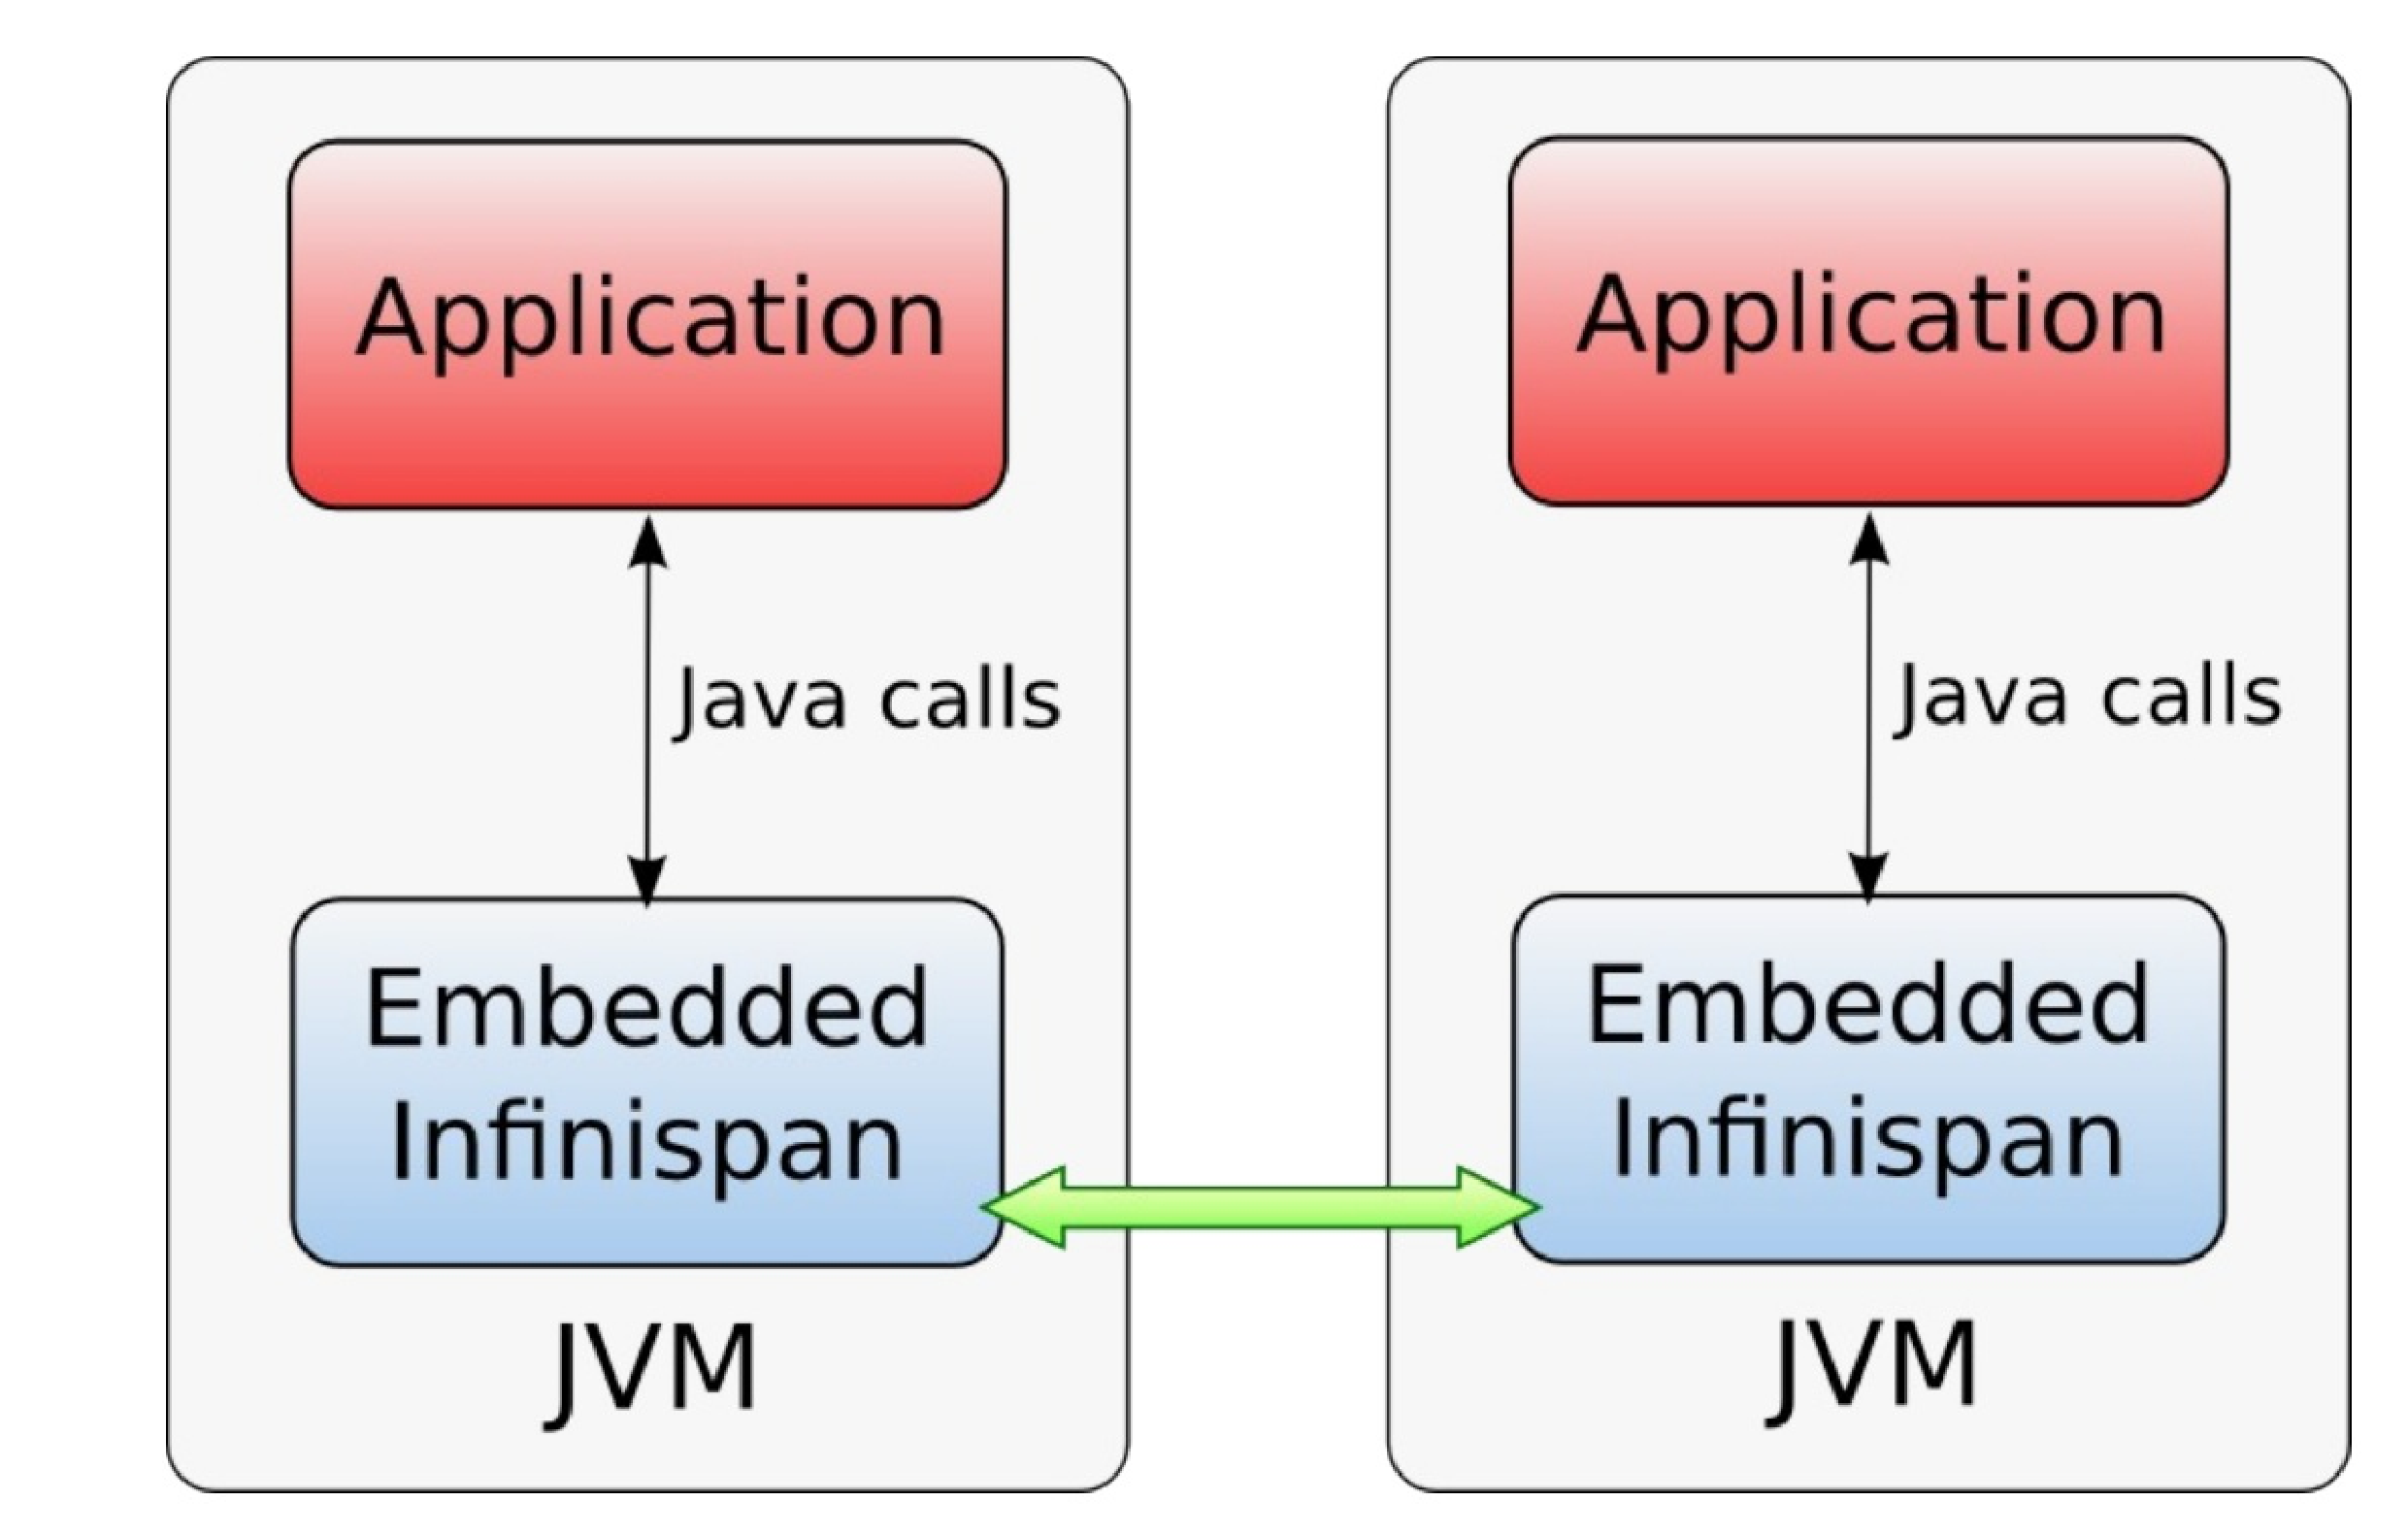
\includegraphics[width=5cm]{./img/ispn-emb.eps}
		\end{figure}
	\column{0.5\textwidth}
		\begin{itemize}
			\item Client-server (remote)
		\end{itemize}
		\begin{figure}
			%\centering
			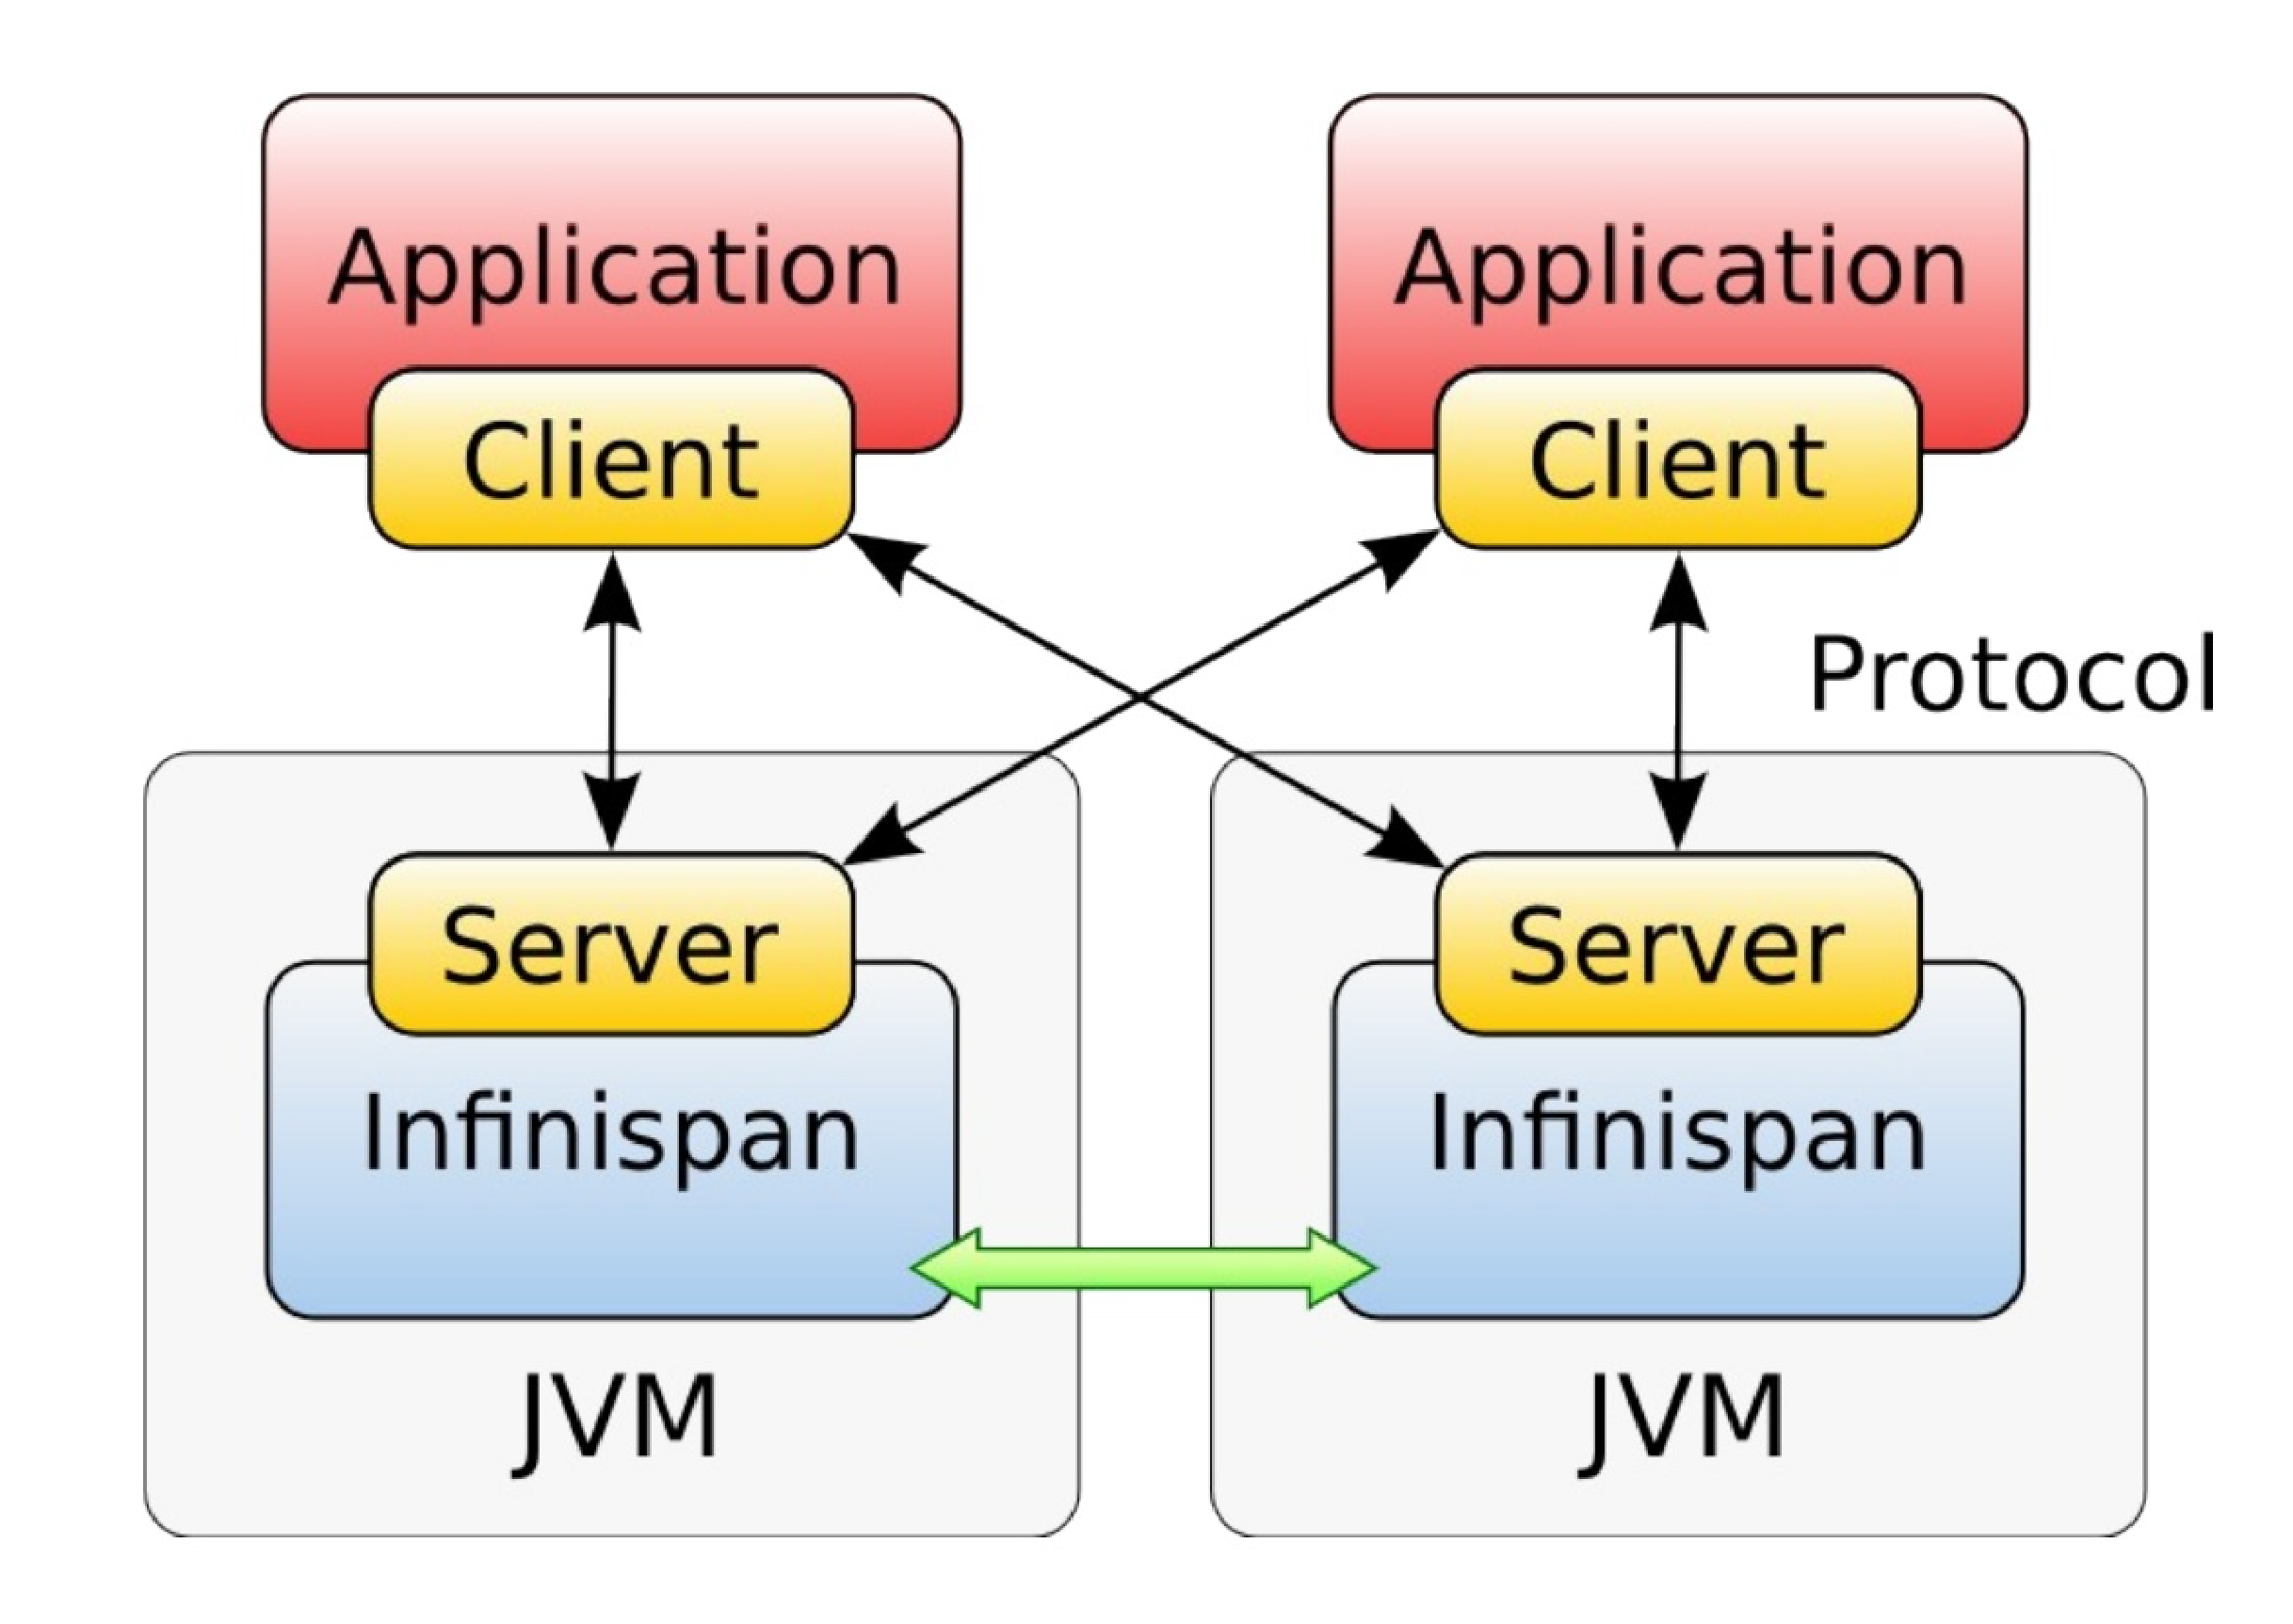
\includegraphics[width=5cm]{./img/ispn-cs.eps}
		\end{figure}
	\end{columns}
\end{frame}

\begin{frame}
	\frametitle{Clustering modes}
	Under the hood leverages JGroups project for clustering.
	\begin{columns}
	\column{0.5\textwidth}
		\begin{itemize}
			\item Local - no clustering
			\vspace{3cm}
			\item Replicated
			\begin{figure}
				%\centering
				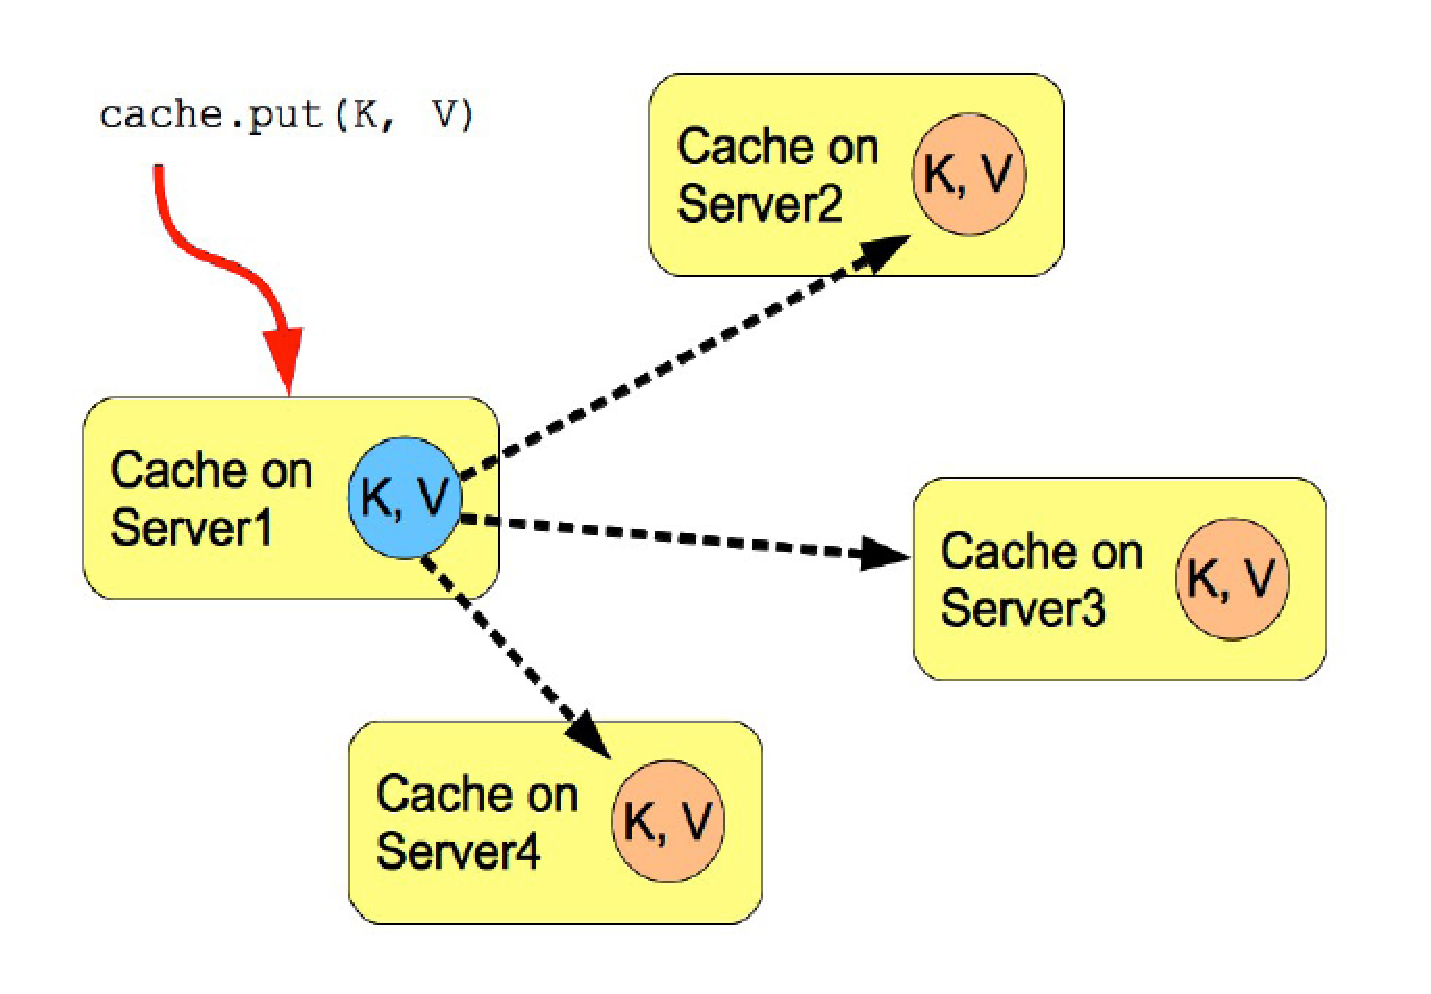
\includegraphics[width=4cm]{./img/ispn-repl.eps}
			\end{figure}
		\end{itemize}
	\column{0.5\textwidth}
		\begin{itemize}
			\item Distributed
			\begin{figure}
				%\centering
				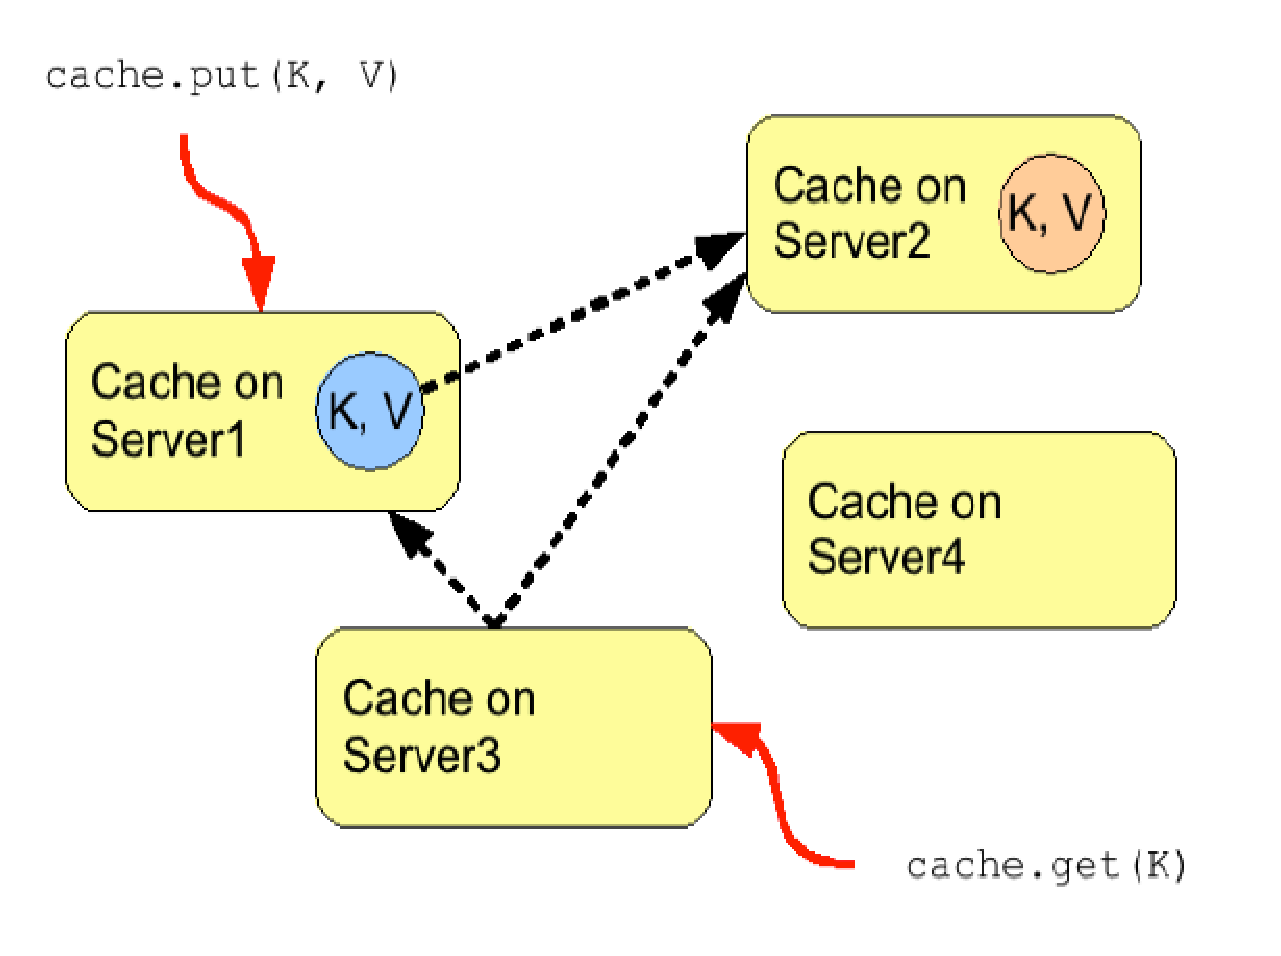
\includegraphics[width=4cm]{./img/ispn-dist.eps}
			\end{figure}
			\item Invalidation
			\begin{figure}
				%\centering
				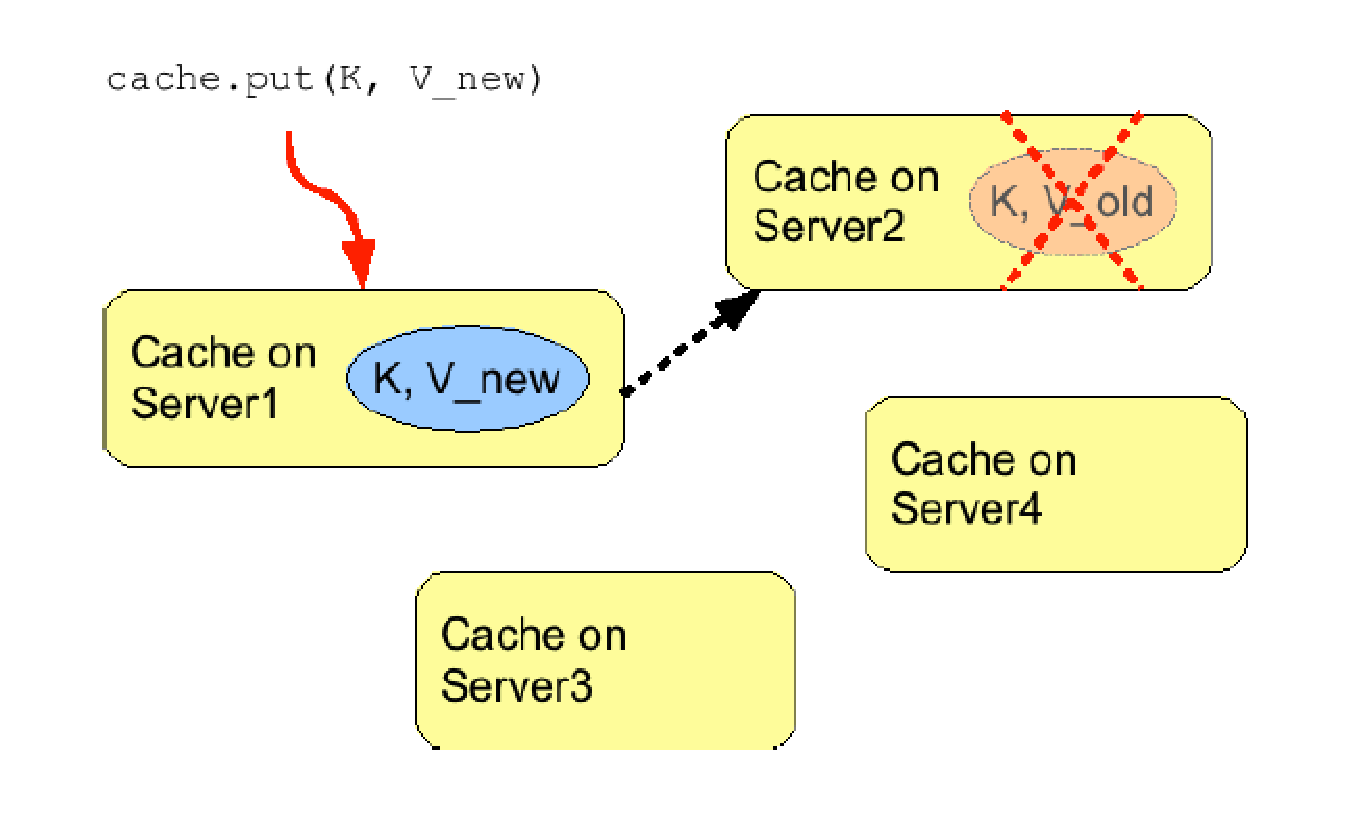
\includegraphics[width=4cm]{./img/ispn-inval.eps}
			\end{figure}
		\end{itemize}
	\end{columns}
\end{frame}


\begin{frame}
	\frametitle{Remote protocols}
	\begin{columns}
	\column{0.5\textwidth}
		\begin{itemize}
			\item HotRod
				\begin{itemize}
					\item hashing and topology aware
					\item failover during topology changes
					\item smart request routing
				\end{itemize}
			\item Memcached
			\item REST
		\end{itemize}
	\column{0.5\textwidth}
		\begin{figure}
			%\centering
			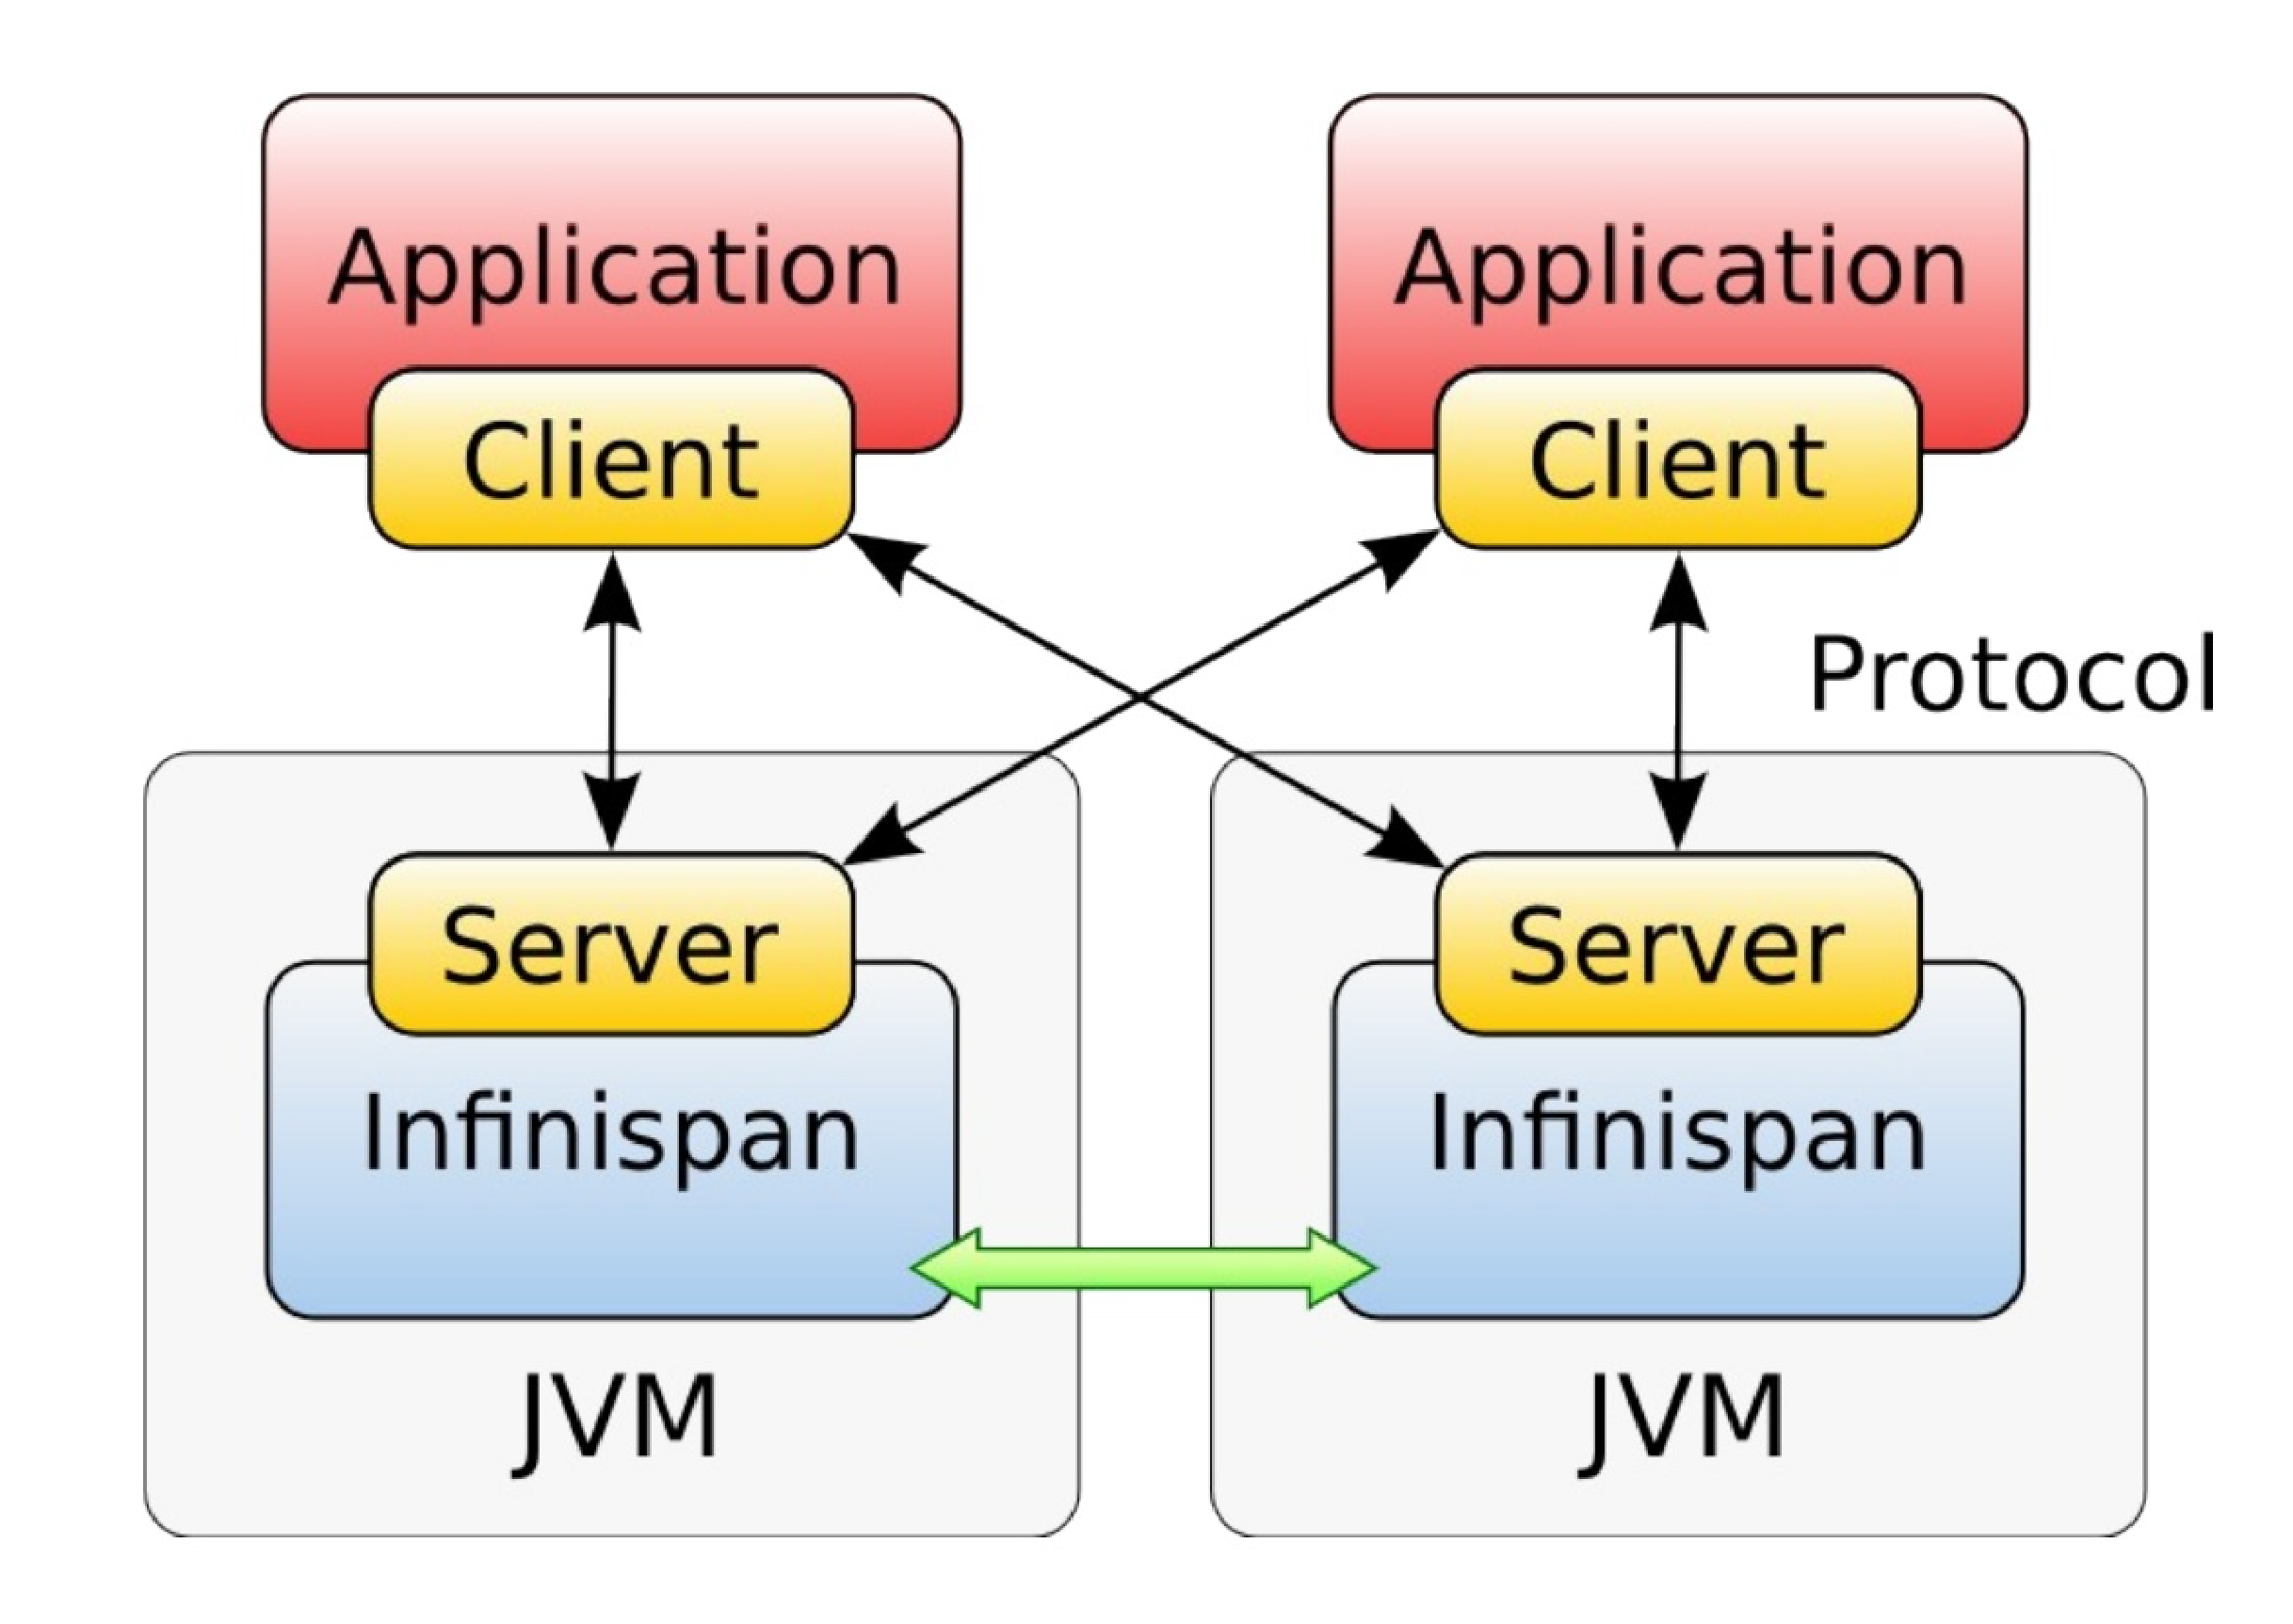
\includegraphics[width=5cm]{./img/ispn-cs.eps}
		\end{figure}
	\end{columns}
\end{frame}

\begin{frame}
  \frametitle{Hotrod clients}
	Compatible with Java and non-Java platforms. Based on Protocol Buffers - Google's data interchange format.\\
	\vspace{0.5cm}
	Clients for
	\begin{itemize}
		\item Java
		\item C\#
		\item C++
		\item Python
		\item Ruby
	\end{itemize}
	Python and Ruby clients have only basic functionality.
\end{frame}

\begin{frame}
	\frametitle{Cache stores}
	A way how to store cache content in some external (persistent) storage.\\
	Two modes:
	\begin{itemize}
	 \item Sychronous (write-through)
	 \item Asynchronous (write-behind)
	\end{itemize}
	Cachestores:
	\begin{itemize}
		\item Single file store and soft-index file store
		\item JDBC and JPA cache stores
		\item LevelDB cache store
		\item Cloud cache store
		\item Remote store
		\item \dots and others
  \end{itemize}
	Also possible to define custom cache store.
\end{frame}

\begin{frame}
	\frametitle{Transactions}
	\begin{itemize}
	 \item Support JTA-compliant transactions
	 \item Ensures consistency of data
	 \item Optimistic and pessimistic locking available
	 \item Read committed and repeated read isolation levels
	 \item Deadlock detection and recovery
	 \item Data versioning
% 		\begin{itemize}
% 			\item Simple versioning
% 			\item Partition-aware versioning (vector locks)
% 			\item External versioning - used e.g. with Hibernate, where locks are provided by database
% 		\end{itemize}
	\end{itemize}
\end{frame}

\begin{frame}
	\frametitle{Querying}
	\begin{itemize}
		\item needs some data schema (annotrations, protobuf, ...)
	 \item Search for data using data attributes instead of keys
	 \item Featured attributes include keyword, range, fuzzy, wildcard, and phrase queries.
	 \item Combine queries and aggregation functions (but doesn't support joins)
	 \item Sort, filter, and paginate query results
	 \item suppor for index or non-indexed queries
	 \item Allows for indexing of entries as they are stored
	 \item Indexing
	 \item Lucene query API or fluent DSL API
	\end{itemize}
\end{frame}

\begin{frame}
	\frametitle{Security}
	\begin{itemize}
	 \item Role based access control
	 \item User authentication
	 \item Node authentication and authorization
	 \item Encryption of communication
	 \item Audit logging
	 \item Integration with LDAP and/or Kerbero server (includes ActiveDirectory)
	\end{itemize}
\end{frame}


\begin{frame}
  \frametitle{Some other features - brief and selective list}
  \begin{itemize}
		\item Data eviction
		\item Full JSR-107 support (Java Temporary Caching API)
		\item CDI support
		\item Remote events
		\item Client near cache
		\item Rolling upgrades
		\item Cross data center replication (separate slide??? With HR failover ability)
		\item Command line interface
		\item Map-reduce framework and distributed executors
  \end{itemize}
\end{frame}


\begin{frame}
  \frametitle{Recently implemented features}
	\begin{figure}
		\centering
		
\includegraphics[width=5cm]{./img/infinispan8.eps}
	\end{figure}
  \begin{itemize}
    \item Functional API
		\item Distributed streaming
		\item Integration with Apache Spark
  \end{itemize}
\end{frame}

\begin{frame}
  \frametitle{Integration with other frameworks}
  \begin{itemize}
    \item Hibernate
		\begin{itemize}
			\item 2-nd level cache
		\end{itemize}
		\item Lucene directory
		\begin{itemize}
		 \item In-memory Lucene index 
		\end{itemize}
		\item Apache Camel
		\begin{itemize}
		 \item Infinispan component for Camel
		\end{itemize}
		\item Hadoop
		\begin{itemize}
			\item In-memory data source for Hadoop cluster
		\end{itemize}
		\item Apache Spark
		\begin{itemize}
			\item Data source for Spark map-reduce jobs
		\end{itemize}
  \end{itemize}
\end{frame}

\begin{frame}
	\centering
	\huge{\textbf{Demo}} \\
	\vspace{1cm}
	\huge{\textbf{Integration with Apache Spark}}
\end{frame}

\begin{frame}
	\frametitle{Some projects using Infinispan}
	\begin{columns}
	\column{0.2\textwidth}
	\column{0.85\textwidth}
		\begin{itemize}
			\item WildFly
				\hspace{10cm}
				\begin{figure}
					\vspace{-1cm}
					
\includegraphics[height=0.75cm]{./img/wildfly.eps}
				\end{figure}
			\item Hibernate
				\hspace{10cm}
				\begin{figure}
					\vspace{-1cm}
					
\includegraphics[height=0.75cm]{./img/hibernate.eps}
				\end{figure}
			\item Apache Camel
				\hspace{10cm}
				\begin{figure}
					\vspace{-1cm}
					
\includegraphics[height=0.75cm]{./img/apache-camel.eps}
				\end{figure}
			\item Apache Marmotta
				\hspace{10cm}
				\begin{figure}
					\vspace{-1cm}
					
\includegraphics[height=0.75cm]{./img/marmotta.eps}
				\end{figure}
			\item CapeDwarf
				\hspace{10cm}
				\begin{figure}
					\vspace{-1cm}
					
\includegraphics[height=0.75cm]{./img/capedwarf.eps}
				\end{figure}
			\item Immutant
				\hspace{10cm}
				\begin{figure}
					\vspace{-1cm}
					
\includegraphics[height=0.75cm]{./img/immutant.eps}
				\end{figure}
			\item apiman
				\hspace{10cm}
				\begin{figure}
					\vspace{-1cm}
					
\includegraphics[height=0.5cm]{./img/apiman.eps}
				\end{figure}
			\item \dots and others
		\end{itemize}
	\end{columns}
\end{frame}


\begin{frame}
	\centering
	\huge{\textbf{Thank you for your attention!}} \\
	\vspace{1cm}
	\huge{\textbf{Questions?}}
\end{frame}

%%%%%%%%%%%%%%%%%%% SOME EXAMPLES %%%%%%%%%%%%%%%%%%%%%%

% \begin{frame}[fragile] %needs to be here to use verbatim
%  \textit{???} \\
%  \vspace{0.3cm}
%  \pause
%  \begin{scriptsize}\url{https://???}\end{scriptsize}
%  \scriptsize{
%    \begin{verbatim}
% wget -O /etc/yum.repos.d/jenkins.repo http://pkg.jenkins-ci.org/redhat/jenkins.repo
% rpm --import http://pkg.jenkins-ci.org/redhat/jenkins-ci.org.key
% yum -y install jenkins
% service jenkins start
%    \end{verbatim}
%  }
%   \begin{columns}
%   \column{0.65\textwidth}
%   \begin{itemize}
%   \item PHP:
% 		\begin{itemize}
% 			\item Check \url{http://jenkins-php.org/} or book \texttt{PHP projects with Jenkins} by O'Reilly
% 		\end{itemize}
%   \pause
%   \item Far not a complete list, list above is just my personal selection of some interesting plugins! Also plugins for other languages exists.
%   
%  \end{itemize}
%  \column{0.33\textwidth}
% 	\begin{figure}
% 		\centering
% 		\includegraphics[width=3cm]{./img/php_book.eps}
% 	\end{figure}
%   \end{columns}
% \end{frame}
% 



% \begin{frame}
% 	\frametitle{Releases, packages}
% 	\begin{columns}
% 		\vspace{-5cm}
% 		\column{0.59\textwidth}
% 		\url{http://jenkins-ci.org}\\
% 		\vspace{1cm}
% 		Release cycle:
% 		\begin{itemize}
% 		 \item Released usually weekly \tikz[na] \coordinate (s_weekly); - release early, release often.
% 		 \item Long term support (LTS) release \tikz[na] \coordinate (s_LTS); - every 3 months, every month minor release with backports of major bug fixes.
% 		\end{itemize}
% 		\vspace{1cm}
% 		
% 		Distribution (Jenkins is a Java servlet):
% 		\begin{itemize}
% 		 \item Web archive (WAR). \tikz[na] \coordinate (s_war);
% 		 \item Native package. \tikz[na] \coordinate (s_native);
% 		\end{itemize}
% 		\vspace{4cm}
% 
% 	
% 		\column{0.4\textwidth}
% 		\vspace{0.5cm}
% 		%\tikzstyle{background grid}=[draw, black!50,step=.5cm]
% 		\begin{tikzpicture}%[show background grid]
%             % Put the graphic inside a node. This makes it easy to place the
%             % graphic and to draw on top of it. 
%             % The above right option is used to place the lower left corner
%             % of the image at the (0,0) coordinate. 
%             \node [inner sep=0pt,above right] 
%                 {\includegraphics[width=8cm]{./img/jenkins_download.eps}};
%             % show origin
%             %\fill (0,0) circle (2pt);
%             % define destination coordinates
%             \path (0.8,10.5) coordinate (weekly)
%                   (2,10.5) coordinate (LTS)
%                   (1.5,10) coordinate (war)
%                   (0.5,7) coordinate (native);
%         \end{tikzpicture}
% 	\end{columns}
% % define overlays
% % Note the use of the overlay option. This is required when 
% % you want to access nodes in different pictures.
% \begin{tikzpicture}[overlay]
%         \path[->,red,thick] (s_weekly) edge [bend left] (weekly);
%         \path[->,blue,thick] (s_LTS) edge [bend left] (LTS);
%         %\path[->,red,thick] (s_war) edge [out=0, in=-90] (war);
%         \path[->,red,thick] (s_war) edge [out=0, in=-90] (war);
%         \path[->,blue,thick] (s_native) edge [out=0, in=-90] (native);
% \end{tikzpicture}
% 
% \end{frame}



\end{document}